\chapter{Combined Algorithm} \label{chapter 4}
Now, we would like to take our discussion one step further. Having explored the spectral algorithm and the greedy recovery algorithm, a natural question arises: can we achieve higher accuracy in the easy regime than the existing solution (i.e., the spectral algorithm) by combining the greedy recovery algorithm with the spectral algorithm? Specifically, if we utilise the assignment computed by the spectral algorithm as the partial seed set for our greedy recovery algorithm, can we improve the accuracy of the spectral algorithm?\\ 
\section{Experimental Results for k=2 in Easy Regime}
\begin{figure}[ht]
    \centering
    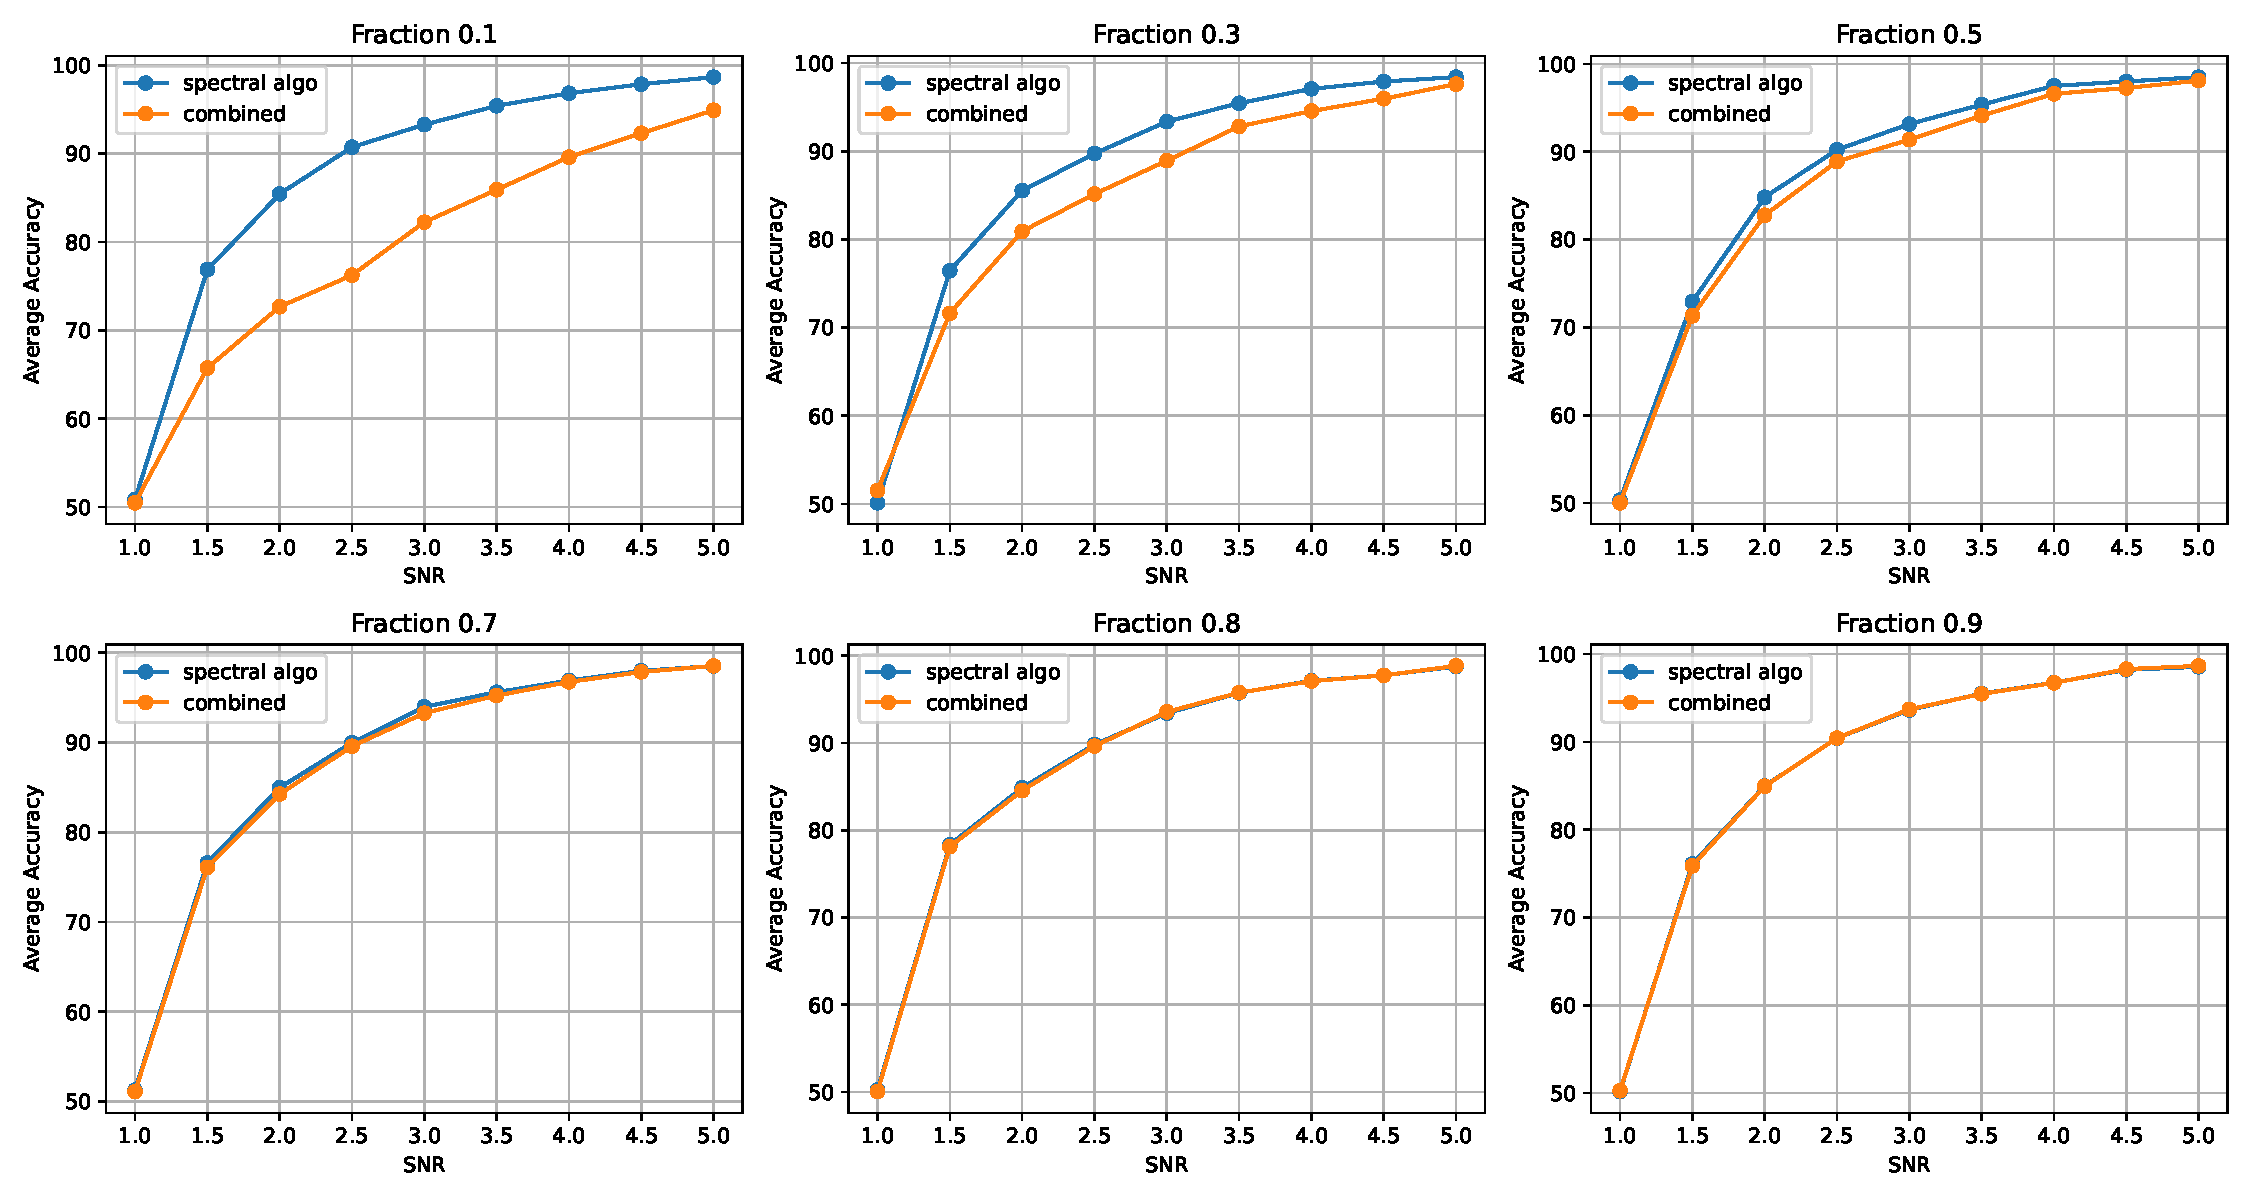
\includegraphics[width=1\linewidth]{Figures/combined_fitting_2.pdf}
    \caption[Combined Algorithm vs Spectral Algorithm]{The blue line represents the accuracy of spectral algorithm, while orange line represents the accuracy of combined algorithm. The experiment results are averaged over 10 instances with $n=10^4$, averge degree $c=6$\protect\footnotemark~and SNR ranging from 1 to 5.}
    \label{fig:combined}
\end{figure}
We randomly select $fraction\times n$ vertices from the assignment computed by spectral algorithm to serve as the partial seed set for the greedy recovery algorithm.  The result is shown in figure \ref{fig:combined}.\\
From this figure, we can observe that the accuracy of the combined algorithm converges to the accuracy of the spectral algorithm as the fraction value increases. Unfortunately, it does not outperform the spectral algorithm. Nevertheless, this finding still inspires a promising direction for future research. If we investigate the assignment computed by the spectral algorithm by utilising some spectral properties of the given graph, can we identify the vertex assignments that are more likely to be correct? By doing so, we may be able to outperform the spectral algorithm in the easy regime.
\footnotetext{In order to test a wide range of SNR values, we have to increase the value of c, as SNR $\leq 3$ for c=3.}